\documentclass[a4paper,12pt]{article} 

\usepackage{multirow}
 \usepackage[table,xcdraw]{xcolor}

%%% Работа с русским языком
\usepackage{cmap}					% поиск в PDF
\usepackage{mathtext} 				% русские буквы в фомулах
\usepackage[T2A]{fontenc}			% кодировка
\usepackage[utf8]{inputenc}			% кодировка исходного текста
\usepackage[english,russian]{babel}	% локализация и переносы

%%% Дополнительная работа с математикой
\usepackage{amsmath,amsfonts,amssymb,amsthm,mathtools, gensymb} % AMS
\usepackage{icomma} % "Умная" запятая: $0,2$    ф--- число, $0, 2$ --- перечисление

%%Таблица
\usepackage[table,xcdraw]{xcolor}
\usepackage{caption}
\usepackage{floatrow}
\floatsetup[table]{capposition=top}
\floatsetup[wrapfigure]{capposition=bottom}

%Отступы и поля 
\textwidth=18cm
\oddsidemargin=-1cm
\topmargin=-2cm
\textheight=25cm


%% Номера формул
\mathtoolsset{showonlyrefs=true} % Показывать номера только у тех формул, на которые есть \eqref{} в тексте.

%% Шрифты
\usepackage{euscript}	 % Шрифт Евклид
\usepackage{mathrsfs} % Красивый матшрифт

%% Свои команды
\DeclareMathOperator{\sgn}{\mathop{sgn}}

%% Перенос знаков в формулах (по Львовскому)
\newcommand*{\hm}[1]{#1\nobreak\discretionary{}
{\hbox{$\mathsurround=0pt #1$}}{}}

%% Стиль страницы
\usepackage{fancyhdr}

%% Для рисунков
\usepackage{graphicx}
\usepackage[export]{adjustbox}
\usepackage{float}
\usepackage{ragged2e}
\usepackage{wrapfig}

\pagestyle{fancy}
\begin{document}
\begin{titlepage}
\begin{center}
%\vspace*{1cm}
\large{\small ФЕДЕРАЛЬНОЕ ГОСУДАРСТВЕННОЕ АВТОНОМНОЕ ОБРАЗОВАТЕЛЬНОЕ\\ УЧРЕЖДЕНИЕ ВЫСШЕГО ОБРАЗОВАНИЯ \\ МОСКОВСКИЙ ФИЗИКО-ТЕХНИЧЕСКИЙ ИНСТИТУТ\\ (НАЦИОНАЛЬНЫЙ ИССЛЕДОВАТЕЛЬСКИЙ УНИВЕРСИТЕТ)\\ ФАКУЛЬТЕТ АЭРОКОСМИЧЕСКИХ ТЕХНОЛОГИЙ}
\vfill
\line(1,0){490}\\[1mm]
\huge{Лабораторная работа 4.2.1}\\
\huge\textbf{Кольца Ньютона}\\
\line(1,0){490}\\[1mm]
\vfill
\begin{flushright}
\normalsize{Рогозин Владимир}\\
\normalsize{\textbf{Группа Б03-106}}\\
\end{flushright}
\end{center}
\end{titlepage}
\fancyhead[L] {Работа 4.2.1}


\textbf{Цель работы}: 
познакомиться с явлением интерференции в тонких плёнках (полосы равной толщины) на примере колец Ньютона и с методикой интерференционных измерений кривизны стеклянной поверхности.


\textbf{Оборудование}:
измерительный микроскоп с опак-иллюминатором; плосковыпуклая линза; пластинка из чёрного стекла; ртутная лампа ДРШ; щель; линзы; призма прямого зрения; объектная шкала.


\textbf{Теоретические сведения}:

\textbf{Интерференция монохроматических волн.}
Пусть в пространстве распространяются две монохроматические
волны одинаковой частоты с амплитудами $a_1$ и $a_2$, и пусть в некоторой
точке наблюдения их фазы равны $\varphi_2$ и $\varphi_1$ соответственно.

\begin{wrapfigure}[15]{l}{0.4\textwidth}\label{fig: Сложение колебаний}
    \begin{center}
    \vspace{-20pt}
        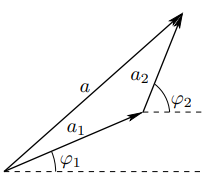
\includegraphics[width = 0.7\textwidth]{Сложение колебаний.png}
    \end{center}
    \caption{Сложение колебаний}
\end{wrapfigure}

Согласно принципу суперпозиции, результирующий колебательный процесс в точке наблюдения представляет собой сумму колебаний, создаваемых каждой из волн, т. е. гармоническое колебание той же частоты $\omega$.  Интенсивность результирующего колебания можно найти используя правило сложения векторов.

\begin{equation}\label{eq: Сложение колебаний}
    I = I_1 + I_2 + 2\sqrt{I_1 I_2}\cos{\Delta \varphi},
\end{equation}

где $\Delta\varphi = \varphi_1 - \varphi_2$ -- разность фаз, $I_1 = a_1^2$ и $I_2 = a_2^2$ -- интенсивности слагаемых волн.

\textit{Интенсивность} -- величина, пропорциональная плотности потока энергии в волне. В пространстве, где налагаются две волны, происходит \textit{перераспределение потоков энергий}: в некоторых точках пространства результирующая интенсивность больше суммы интенсивностей слагаемых волн, в других точках, наоборот, результирующий поток энергии меньше суммы потоков энергии в слагаемых волнах. Это явление называется \textbf{\textit{интерференцией}}. При наложении волн одинаковой интенсивности $I_1 = I_2 = I_0$ имеем 
\begin{equation}\label{eq: Сложение колебаний I_1 = I_2}
    I = 2 I_0(1 + \cos{\Delta \varphi}).
\end{equation}
Чередующиеся максимумы $I_{max}$ и минимумы $I_{min}$ результирующей интенсивности образуют интерференционные полосы.

\textbf{Двухлучевая интерференция.}  
В любой двухлучевой интерференционной схеме свет от одного источника приходит в точку наблюдения по двум различным путям $r_1$ и $r_2$ с разностью фаз $\Delta\varphi = k_2r_2 - k_1r_1$, где $k_1 = n_1 \omega / c$ и $k_2 = n_2 \omega / c$ (частота волны при переходе из одной среды в другую остаётся неизменной). Таким образом,
\begin{equation}\label{eq: Разность фаз двухлучевой интерференции}
    \varphi_2 - \varphi_1 = \frac{\omega}{c}(n_2r_2 - n_1r_1) = \frac{\omega}{c} \cdot \Delta,   
\end{equation}
где $n_1$ и $n_2$ -- \textit{показатели преломления} среды вдоль путей $r_2$ и $r_1$ соответственно. 
\begin{equation}\label{eq: Разность оптических путей}
    \Delta = n_2r_2 - n_1r_1
\end{equation}
есть разность \textit{оптических путей} двух плеч интерферометра (\textit{оптическая разность хода}). 

Если амплитуды волн в точке наблюдения одинаковы, то получаем 
\begin{equation}\label{eq: Интенсивность через оптическую разность хода}
    I = 2I_0 (1 + \cos{\frac{\omega}{c} \Delta}).
\end{equation}
Эта формула справедлива при интерференции любых монохроматических волн одинаковой частоты и интенсивности.

\textbf{Видность.}
Контраст интерференционной картины принято характеризовать величиной \textit{видности} $\nu$, определяемой равенством
\begin{equation}\label{eq: Видность}
    \nu = \frac{I_{max} - I_{min}}{I_{max} + I_{min}}.
\end{equation}
Интенсивность максимальна и равна $I_{max} = (a_1 + a_2)^2$ при $\Delta\varphi = 2m \pi$, где $m$ -- целое число, называемое порядком интерференции. Геометрическое место точек, удовлетворяющих этим условиям, образует максимумы (светлые интерференционные полосы) m-го порядка. $\Delta\varphi = (2m + 1) \pi$ возникают минимумы (тёмные интерференционные полосы). Видность максимальна (и равна единице) при равных амплитудах волн, при этом $I_{max} = 4 I_0$ вдвое больше суммы интенсивностей
слагаемых волн, а $I_{min} = 0$.

\textbf{Кольца Ньютона.} 
Этот классический опыт используется для определения \textit{радиуса кривизны} сферических поверхностей линз. В этом опыте наблюдается интерференция волн, отражённых от границ тонкой воздушной прослойки, образованной сферической поверхностью линзы и плоской стеклянной пластиной. При нормальном падении света интерференционные полосы локализованы на сферической поверхности и являются полосами равной толщины.

\begin{wrapfigure}[16]{l}{0.4\textwidth}\label{fig: Линза на пластине}
    \begin{center}
    \vspace{-20pt}
        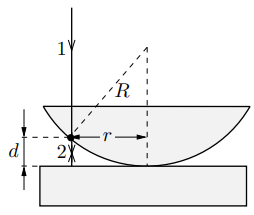
\includegraphics[width = 0.9\textwidth]{Линза на пластине.png}
    \end{center}
    \caption{ Схема наблюдения
колец Ньютона}
\end{wrapfigure}
Геометрическая разность хода между интерферирующими лучами равна удвоенной толщине воздушного зазора $2d$ в данном месте. Для точки на сферической поверхности, находящейся на расстоянии $r$ от оси системы, имеем $r^2 = R^2 - (R - d)^2 = 2Rd - d^2$, где $R$ -- радиус кривизны сферической поверхности. При $R\gg d$ получим $d = r^2/2R$. С учётом изменения фазы на $\pi$ при отражении волны от оптически более плотной среды (на границе воздух—стекло) получим оптическую разность хода интерферирующих лучей:
\begin{equation}\label{eq: Оптическая разность хода для колец Ньютона}
    \Delta = 2d + \frac{\lambda}{2} = \frac{r^2}{R} + \frac{\lambda}{2}.
\end{equation}
Условие интерференционного минимума есть $\Delta = (2m + 1) \frac{\lambda}{2}$ ($m$ = 0, 1, 2, . . .), откуда
получаем для радиусов тёмных колец
\begin{equation}\label{eq: Радиусы темных колец}
    r_m = \sqrt{m \lambda R}.
\end{equation}
Аналогично для радиусов $r'_m$ светлых колец

\begin{equation}\label{eq: Радиусы светлых колец}
    r'_m = \sqrt{(2m - 1) \lambda R / 2}.
\end{equation}

\begin{figure}[H]\label{fig: Отражение лучей от стекла}
    \centering
    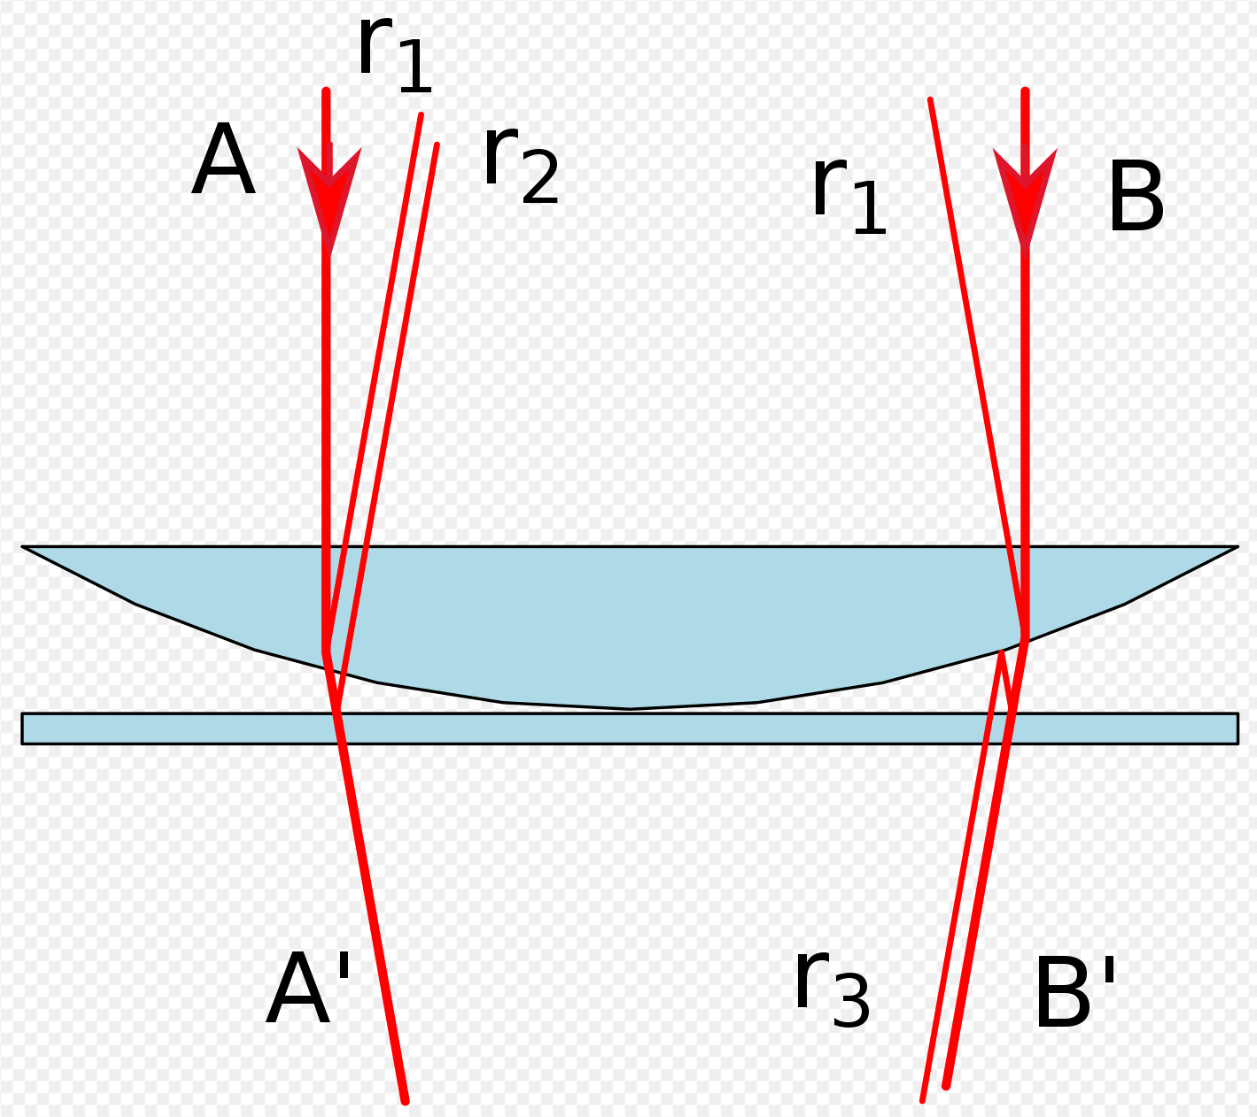
\includegraphics[width = 0.8\textwidth]{Отражение лучей от стекла.png}
    \caption{Образование колец Ньютона в отражённом (слева) и в проходящем свет (справа)}
\end{figure}

\textbf{Экспериментальная установка}:

Схема экспериментальной установки приведена на рис. 4. Опыт выполняется с помощью измерительного микроскопа. На столике микроскопа помещается держатель с пластинкой чёрного стекла. На пластинке лежит исследуемая линза.

\begin{figure}[H]\label{fig: Установка}
    \centering
    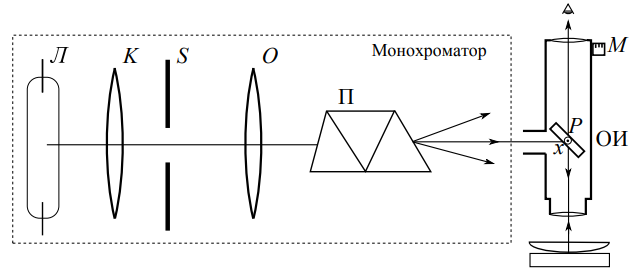
\includegraphics[width = 0.9\textwidth]{Установка.png}
    \caption{Схема установки для наблюдения колец Ньютона}
\end{figure}

Источником света служит ртутная лампа, находящаяся в защитном кожухе. Для получения монохроматического света применяется призменный монохроматор, состоящий из конденсора $K$, коллиматора (щель $S$ и объектив $O$) и призмы прямого зрения $\Pi$. Свет от
монохроматора попадает на опак-иллюминатор (ОИ), расположенный между окуляром и объективом микроскопа -- специальное устройство для освещения объекта при работе в отражённом свете. Внутри опакиллюминатора находится полупрозрачная пластинка $P$, наклоненная под углом 45\degree{} к оптической оси микроскопа. Свет частично отражается от этой пластинки, проходит через объектив микроскопа и попадает на исследуемый объект.

Столик микроскопа может перемещаться в двух взаимно перпендикулярных направлениях с помощью винтов препаратоводителя. Отсчетный крест окулярной шкалы перемещается перпендикулярно оптической оси микроскопа с помощью микрометрического винта $M$. 

Оптическая схема монохроматора позволяет получить в плоскости входного окна опак-иллюминатора достаточно хорошо разделённые линии спектра ртутной лампы. Изображение щели $S$ фокусируется на поверхность линзы объективом микроскопа, и в том же месте находится плоскость наблюдения микроскопа, т. е. точка источника и точка наблюдения интерференции совпадают. Картина интерференции как и в случае расположения пластинки сверху, так и в данном случае не зависит от коэффициента преломления линзы и определяется величиной зазора между нижней поверхностью линзы  и стеклянной пластинкой.

\textbf{Обработка данных}:  
\begin{enumerate}
    \item Рассчитаем цену деления окулярной шкалы. Для этого сверху на линзу положим калиброванную объектную шкалу, найдём её изображение и совместим его с окулярной шкалой. Объектная шкала размером 1 мм разбита на 100 делений, т.е. её цена деления равна 0,01 мм. Теперь совместим две шкалы так, чтобы штрихи объектной шкалы лучше всего совпадали со штрихами окулярной шкалы. Запишем значение и рассчитаем коэффициент $k$ перевода делений окулярной шкалы в миллиметры:
    \[(4,90 - 3,88) \text{ дел.} = 0,1 \text{ мм } (\text{10 делений.})\]
    \[k = \frac{10^{-1}}{1,02} \text{ } \frac{мм}{дел.} \approx 9,8 \cdot 10^{-2} \frac{мм}{дел.}.\]
    Абсолютная погрешность измерения радиусов колец равна половине наименьшего расстояния между соседними полосами, т.е. 
    \[\sigma_x = 9,8 \cdot 10^{-2} \cdot \frac{7}{200} \text{ мм} \approx 3,43 \cdot 10^{-3} \text{ мм}.\]
    \item Далее будем идти от одного достаточно удалённого кольца к центру и снимать по окулярной шкале значения положений центров колец. Дойдя до центра центрального пятна, запишем его положение и будем продолжать измерение координат центров колец с другой стороны от пятна. Результаты измерений приведены в таблице ниже.

    Радиус кольца можно рассчитать трёмя способами:  1) используя координаты концов кольца; 2) используя координаты левого конца и центра центрального пятна; 3) используя координаты правого конца и центра центрального пятна. В данной работе радиус кольца рассчитывается каждым из способов, затем берётся среднее арифметическое по трём значениям. При этом абсолютная погрешность значения радиуса вычисляется по формуле
    \[\sigma_r = \sqrt{2} \cdot \sigma_x \approx 4,85 \cdot 10^{-3} \text{ мм.}\]

    \begin{table}[H]\label{tab: right and left}
        \centering
        \begin{tabular}{|
            >{\columncolor[HTML]{FFFFFF}}c |
            >{\columncolor[HTML]{FFFFFF}}c |
            >{\columncolor[HTML]{FFFFFF}}c |
            >{\columncolor[HTML]{FFFFFF}}c |}
            \hline
            {\color[HTML]{000000} Номер кольца m} & {\color[HTML]{000000} Цвет кольца} & {\color[HTML]{000000} Левый край, дел.} & {\color[HTML]{000000} Правый край, дел.} \\ \hline
            \cellcolor[HTML]{FFFFFF}{\color[HTML]{000000} }                    & {\color[HTML]{000000} Светлый} & {\color[HTML]{000000} 4,19} & {\color[HTML]{000000} 5,49} \\ \cline{2-4} 
            \multirow{-2}{*}{\cellcolor[HTML]{FFFFFF}{\color[HTML]{000000} 1}} & {\color[HTML]{000000} Темный}  & {\color[HTML]{000000} 3,99} & {\color[HTML]{000000} 5,73} \\ \hline
            \cellcolor[HTML]{FFFFFF}{\color[HTML]{000000} }                    & {\color[HTML]{000000} Светлый} & {\color[HTML]{000000} 3,72} & {\color[HTML]{000000} 5,92} \\ \cline{2-4} 
            \multirow{-2}{*}{\cellcolor[HTML]{FFFFFF}{\color[HTML]{000000} 2}} & {\color[HTML]{000000} Темный}  & {\color[HTML]{000000} 3,57} & {\color[HTML]{000000} 6,10} \\ \hline
            \cellcolor[HTML]{FFFFFF}{\color[HTML]{000000} }                    & {\color[HTML]{000000} Светлый} & {\color[HTML]{000000} 3,41} & {\color[HTML]{000000} 6,23} \\ \cline{2-4} 
            \multirow{-2}{*}{\cellcolor[HTML]{FFFFFF}{\color[HTML]{000000} 3}} & {\color[HTML]{000000} Темный}  & {\color[HTML]{000000} 3,29} & {\color[HTML]{000000} 6,36} \\ \hline
            \cellcolor[HTML]{FFFFFF}{\color[HTML]{000000} }                    & {\color[HTML]{000000} Светлый} & {\color[HTML]{000000} 3,18} & {\color[HTML]{000000} 6,49} \\ \cline{2-4} 
            \multirow{-2}{*}{\cellcolor[HTML]{FFFFFF}{\color[HTML]{000000} 4}} & {\color[HTML]{000000} Темный}  & {\color[HTML]{000000} 3,08} & {\color[HTML]{000000} 6,63} \\ \hline
            \cellcolor[HTML]{FFFFFF}{\color[HTML]{000000} }                    & {\color[HTML]{000000} Светлый} & {\color[HTML]{000000} 3,00} & {\color[HTML]{000000} 6,72} \\ \cline{2-4} 
            \multirow{-2}{*}{\cellcolor[HTML]{FFFFFF}{\color[HTML]{000000} 5}} & {\color[HTML]{000000} Темный}  & {\color[HTML]{000000} 2,86} & {\color[HTML]{000000} 6,82} \\ \hline
            \cellcolor[HTML]{FFFFFF}{\color[HTML]{000000} }                    & {\color[HTML]{000000} Светлый} & {\color[HTML]{000000} 2,77} & {\color[HTML]{000000} 6,92} \\ \cline{2-4} 
            \multirow{-2}{*}{\cellcolor[HTML]{FFFFFF}{\color[HTML]{000000} 6}} & {\color[HTML]{000000} Темный}  & {\color[HTML]{000000} 2,68} & {\color[HTML]{000000} 6,99} \\ \hline
        \end{tabular}
        \caption{Координаты левого и правого концов колец}
    \end{table}
    Координата центра центрального пятна: $X_c = 4,84$ дел.

    Ниже в таблице представлены значения радиусов для каждого из колец.
    \begin{table}[H]\label{tab: r and r}
        \centering
        \begin{tabular}{|
            >{\columncolor[HTML]{FFFFFF}}c |
            >{\columncolor[HTML]{FFFFFF}}c |
            >{\columncolor[HTML]{FFFFFF}}c |
            >{\columncolor[HTML]{FFFFFF}}c |
            >{\columncolor[HTML]{FFFFFF}}c |
            >{\columncolor[HTML]{FFFFFF}}c |
            >{\columncolor[HTML]{FFFFFF}}c |
            >{\columncolor[HTML]{FFFFFF}}c |}
            \hline
            {\color[HTML]{000000} Номер кольца m} &
              {\color[HTML]{000000} 1} &
              {\color[HTML]{000000} 2} &
              {\color[HTML]{000000} 3} &
              {\color[HTML]{000000} 4} &
              {\color[HTML]{000000} 5} &
              {\color[HTML]{000000} 6} &
              {\color[HTML]{000000} Центральное пятно} \\ \hline
            {\color[HTML]{000000} $r_m$, дел.} &
              {\color[HTML]{000000} 0,87} &
              {\color[HTML]{000000} 1,27} &
              {\color[HTML]{000000} 1,54} &
              {\color[HTML]{000000} 1,78} &
              {\color[HTML]{000000} 1,98} &
              {\color[HTML]{000000} 2,16} &
              \cellcolor[HTML]{FFFFFF}{\color[HTML]{000000} } \\ \cline{1-7}
            {\color[HTML]{000000} $r'_m$, дел.} &
              {\color[HTML]{000000} 0,65} &
              {\color[HTML]{000000} 1,10} &
              {\color[HTML]{000000} 1,41} &
              {\color[HTML]{000000} 1,66} &
              {\color[HTML]{000000} 1,86} &
              {\color[HTML]{000000} 2,08} &
              \multirow{-2}{*}{\cellcolor[HTML]{FFFFFF}{\color[HTML]{000000} 0,50}} \\ \hline
        \end{tabular}
        \caption{Радиусы колец}
    \end{table}
    По данным из таблицы построим графики зависимости $r^2_m$ и $(r'_m)^2$ от номера $m$ кольца. Также, на графике отметим границы центрального тёмного пятна.

    По данным из графика, зная коэффициенты наклона прямых, определим радиус кривизны линзы по формуле 
    \[k = \lambda R \Rightarrow R = \frac{k}{\lambda}\]
    где $\lambda$ -- длина волны зелёного света, $k$ -- среднее арифметическое коэффициентов наклона для темных и светлых колец.
    \[R = \frac{k}{\lambda} = \frac{74,3}{5,46} \text{ мм} \approx 13,61 \text{ мм}.\]
    
    \item В третьем пункте будем освещать линзу сразу двумя различными спектральными компонентами ртути (жёлтым и зелёным). В микроскоп будет видна картина «биений»: чёткость интерференционных колец периодически изменяется, за чёткими кольцами следуют более размытые, за которыми потом снова следуют чёткие и т.д. Это объясняется наложением двух систем интерференционных колец, возникающих для разных длин волн $\lambda_1$ и $\lambda_2$. Чёткие кольца в результирующей картине образуются при наложении светлых колец на светлые и тёмных на тёмные. Размытые кольца получаются при наложении светлых колец одной картины на тёмные кольца другой.

    Рассчитать период возникших биений можно используя тот факт, что если в промежутке между двумя центрами соседних чётких участков укладывается $\Delta m$ колец для спектральной линии с длиной волны $\lambda_1$, то  в этом промежутке должно располагаться $(\Delta m - 1)$  колец для спектральной линии с длиной волны $\lambda_2$ (при $\lambda_2 > \lambda_1$). Тогда, для периода биений $\Delta m$ получаем формулу
    \[r^2 = \lambda_1 m_1 R = \lambda_2 m_2 R,\]
    \[(r')^2 = \lambda_1 m'_1 R = \lambda_2 m'_2 R,\]
    \[\lambda_1 \cdot (\Delta m + 1) = \lambda_2 \cdot \Delta m,\]
    \[\Delta m = \frac{\lambda_1}{\lambda_2 - \lambda_1}.\]
    гдe $\lambda_1$ -- длина волны зелёного света. Отсюда получаем выражение для разности длин волн.
    \[\lambda_2 - \lambda_1 = \frac{\lambda_1}{\Delta m}.\]
    Считая темные кольца, находим: $\Delta m = 14$. Теперь найдём разность длин волн, сравним результат с табличным.   
    \begin{table}[H]\label{tab: results lmbd diff}
        \centering
        \begin{tabular}{|
            >{\columncolor[HTML]{FFFFFF}}c |
            >{\columncolor[HTML]{FFFFFF}}c |
            >{\columncolor[HTML]{FFFFFF}}c |}
            \hline
            {\color[HTML]{000000} Номер кольца m}            & {\color[HTML]{000000} Табличное значение} & {\color[HTML]{000000} Экспериментальное значение} \\ \hline
            {\color[HTML]{000000} $\lambda_2 - \lambda_1$, нм} & {\color[HTML]{000000} 1 - 50}             & {\color[HTML]{000000} 39,0}                      \\ \hline
        \end{tabular}
        \caption{Результат измерения разности длин волн}
    \end{table}
    
    
\end{enumerate}



\textbf{Вывод}: В данной работе было изучено явление интерференции электромагнитных волн видимого диапазона на примере колец Ньютона. С помощью интерференции волн рассчитали радиус кривизны линзы ($R \approx 13,61$ мм), а также вычислили и сравнили с табличным значение разности длин волн для желтого и зеленого света ($\Delta \lambda_{эксп.} = 39,0$ нм; \text{ } $\Delta \lambda_{теор.}$ находится в диапазоне $1-50$ нм). Получившийся результат лежит в диапазоне теоретической оценки.

%%%%%%%%%%%%%%%%%%%%%%%%% Графики
\newpage
\begin{figure}[H]\label{fig: r2_r'2(m)}
    \centering
    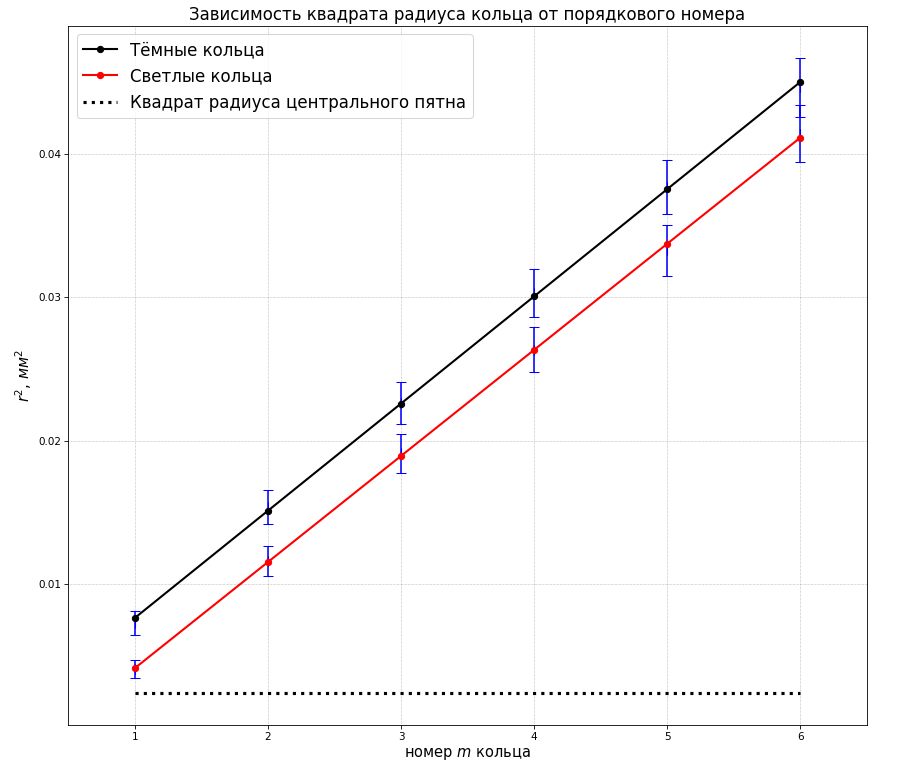
\includegraphics[width = \textwidth]{r2_r'2(m).png}
\end{figure}
Относительная погрешность $r^2$ вычисляется по формуле 
\[\varepsilon_{r^2} = 2 \cdot \varepsilon_r,\]
тогда абсолютная погрешность получается равной
\[\sigma_{r^2} = 2r \cdot \sigma_r.\]
Коэффициенты наклона прямых и их погрешности представлены ниже: 
\[k_{темн.} = (7,467 \pm  0,063) \cdot 10^{-3} \text{ } мм^2, \quad \varepsilon_{k_{темн.}} \approx 0,84 \%;\]
\[k_{светл.} = (7,391 \pm  0,057) \cdot 10^{-3} \text{ } мм^2, \quad \varepsilon_{k_{светл.}} \approx 0,77 \%;\]


%%%%%%%%%%%%%%%%%%%%%%%%%
\end{document}
